% observation
There is a rapid growth in the number of available biological datasets due to
the decreaseing cost of data collection. This brings opportunities to gain novel
insights to the underlying biological mechanisms in the development and
progression of diseases such as cancer, possibly leading to the development of
novel diagnostic tests or drugs for treatment.  The wide range of different
biological datasets has led to the development of a wealth of software packages
and systems to explore and analyze these datasets.  However, there are few tools
that are designed with the full analysis pipeline in mind, from raw data into
interpretable results.  While the tools are used to provide novel insights in
diseases, there is little emphasis on reporting and sharing information about
tool versions, input parameters, and other information that can help others use
the same known methods on their own datasets.  This leads to unnecessary
difficulties to reuse known methods, and difficulties in reproducing analyses,
which leads to longer analysis times and therefore unrealized potential for
scientific insights.

% challenge
There are several 
% LAB: computational challenges in reducing the "analysis time". MEn analysis
% time høres ut som kjøretid.
computational challenges 
% LAB: er noe som er rart med språket her. Eventuelt er det bare jeg som synes
% det
for researchers to analyze
and explore biological datasets. These challenges are common for large datasets
such as high-throughput sequencing data that require long-running, deep analysis
pipelines, as well as smaller datasets, such as microarray data, that require
complex, but short-running analysis pipelines. The first is the time and
knowledge required to find and set up the necessary analysis tools to start
analyzing a modern biological dataset. The second is ensuring the correct input
parameters, tool versions, database versions, and dataset versions when
analyzing, and reporting analysis results to enable reproducible science. A
third challenge is efficiently exploring the results of the analyses
interactively. This includes developing tools that can efficiently visualize the
heterogeneous datsets and integrate them with known biology from databases to
provide necessary information for interpreting the results. The final challenge
is reusing the analysis pipelines and exploration tools with new datasets,
methods, and research questions. 

As a result, there are a wealth of specialized approaches and systems 
to analyze complex biological data. To develop deep analysis pipelines in
bioinformatics, Galaxy\cite{galaxy} has for a long time provided a simple
interface to set up and execute analysis pipelines for genomic datasets.
However, the Galaxy system is less effective for explorative and flexible
analyses where it is necessary 
% LAB: Ikke helt sikker på om jeg er enig i at dette er vanskelig. Er ett tools
% først i Galaxy toolshed tror jeg det er forholdsvis enkelt å teste
% forskjellige konfigurasjoner. Jeg mener det store problement med Galaxy, og
% grunnen til at mange ikke bruker det inkludert oss, er at det er vanskelig å
% skrive nye tools. Det er ett viktig poeng å få frem siden en av de gode
% tingene her er at R er så godt støttet.
to try out different tools with different
configurations.\cite{spjuth2015experiences} New initiatives such as the
\gls{cwl} provide users a standardized way of describing and sharing an analysis
pipeline, and has multiple implementations such as the reference implementation
cwl\_runner,\footnote{\url{github.com/common-workflow-language/cwltool}}
Arvados,\cite{arvados} Rabix,\cite{rabix} Toil,\cite{toil} Galaxy,\cite{galaxy}
and AWE.\cite{awe}
While these systems provide a viable option for batch-processing of
large biological datasets, researchers with smaller datasets at hand, can
analyze and explore them through interactive languages and interpreters such as
Python or the  R programming language. Through the package repository
Bioconductor, there are a wide range of R packages to analyze biological
datasets. These include tools for both analyzing and visualizing the datasets.
For users with little or no programming experience it is possible to access and
explore datasets thorough applications using the Shiny or OpenCPU frameworks.
These let developers write applications in the R programming language, and users
can access and explore the data through web applications. Standalone systems
such as Cytoscape provide a specialized software platform to visualize and
explore complex biological datasets.\cite{cytoscape} 
Generalized systems for analyze a wide range of big datasets are now starting to
get attention in bioinformatics. An example of one of these is Pachyderm, a
system for deploying and managing multi-stage, lagnuage-agnostic data
pipelines.\cite{pachyderm} In addition to tracking pipeline configrations,
it also provides full provenance for the data.
Another example is Aparche Spark, an analytics engine for large-scale data
processing.\cite{spark}. Both of these provide useful abstractions for
reproducible analyses of large-scale datasets, but they have yet to see
wide-spread adpotion in Bioinformatics.  
With the addition of new datasets and methods every year, it seems that analysis
of biological data requires a wide array of different tools and systems.

% our solution
This dissertation argues that, instead, we can design a unified approach that
integrates disperate systems and data into fully reproducible biological data
analysis frameworks. In particular, we show how software container technologies
together with well-defined interfaces, configurations, and orchestration provide
the necessary foundation to build reproducible analysis pipelines for biological
datasets, as well as highly interactive data exploration applications.
% LAB: Synes du at poengene med "easy to develop" og "specialized analyzes" bør
% være med? Enten her, eller i listen nedenfor.

The resulting approach as several key advantages when implementing systems to
analyze and explore biological data:
% LAB: Alle advantages (andre setning) er skrevet for utviklere. Men hva er
% fordelen for sluttbrukere?
\begin{itemize} 
    \item It enables reproducible research by packaging applications
        and tools within containerized environments. This enables sharing of
        tools and simplifies 
        % LAB: tedious er ett problem. Ett annet er at det sikrer at rett
        % versjon av en pipeline er innstalert. Dette er særlig viktig i feks
        % META-pipe, men også for medisinske diagnoser
        the tedious task of installing specific tools. 

    \item It simplifies the sharing of analysis pipelines and workflows across
        different research teams and systems. 
        % LAB: Jeg og mange andre ser ikke hvofor dette shortens...
        This shortens the
        time-to-interpretation for biological datasets. 

    \item It enables applications to use tools written in any programming
        language, using open standards to communicate between tools and systems.
        This allows for exploration tools to interface with both statistical
        analyses and biological databases. % evt. kutte siste setning...
        
    \item It facilitates the development of flexible and configurable systems by
        separating appliications and tools into small composable parts. This
        allows developers to reuse parts of a system to fit new methods and
        datasets. 
\end{itemize} 

From collaboration with researchers in systems epidemiology and precision
medicine we were asked to develop a set of applications and systems that could
enable them to analyze and explore their datasets. From these systems we
extraplolated a set of general design principles to form a unified approach. 
We implement our approach thorugh a series of applications and tools built on
top of a stack of open source systems with software containers as the common
foundation. We evaluate the approach through these systems using real datasets
and show its viability. 

From a longer-term perspective we discuss the general patterns for implementing
modern data analysis systems for use 
% LAB: var veldig spesifisert long-term perspektive, kanskje bedre med en such
% as prec. med.
in precision medicine and dicuss why our
approach is a suitable option. As more datasets are produced every year,
research will depend on systems being 
% LAB: hva er easy to pick up i systems context?
easy to pick up, and provide the necessary
functionality to reproduce and share the analysis pipelines. 

\emph{Thesis statement}:
A unified development model based on software container infrastructure can
efficiently provide reproducible and easy to use environments to develop
applications for exploring and analyzing biological datasets. 

\section{Problems with Data Analysis and Exploration in Bioinformatics}
Today there is a move towards using more sophisticated approaches to analyze
biological datasets through workflow and pipeline mangers such as
Galaxy\cite{galaxy} and the \gls{cwl}\cite{cwl}. These simplify setting up the
analysis pipeline pipeline, maintaining, and updating it. However, these tools
still have their limitations and shell scripts are still the de facto standard
building analysis pipelines in bioinformatics. 
For exploring biological data there are a range of tools, such as
Cytoscape\cite{cytoscape} and Circos\cite{circos},
% more tools? other tools? 
% LAB: virker som Snakemake er populært ihvertfall på NTNU, men også andre
% steder
that support importing an already-analyzed dataset to visualize and browse the
data. 

Although there are efforts to develop tools to help researchers explore and
analyze biological datasets, they current tools have several drawbacks:

\begin{enumerate}
    \item \textbf{Reusability:} Data exploration tools are often
        developed as a single specialized application, making it difficult to
        reuse parts of the application for other analyses or datasets. This
        leads to duplicate development effort and abandoned projects. 
    \item \textbf{Decoupling:} Data exploration tools are often decoupled from
        the statistical analyses. This often makes it a difficult to document
        and retrace the analyses behind the results. 
    \item \textbf{Complexity:} 
        Analyses that start as a simple script quickly become more complex to
        maintain and develop as developers add new functionality to the
        analyses. % vet ikke med denne, mangler noe her. 
        % LAB: kan stjele argumentasjon fra ADAM paperet der de kritiserer
        % "monolothic" bio applikasjoner. Eller fra Tanenbaum vs Linus.
    \item \textbf{Reproducibility:} While there are tools for analyzing most
        data types today, there is little or no effort to fully document the
        entire 
        % LAB: pipeline blir feil her siden du også inkluderer interpretation.
        % Som er ett viktig poeng.
        pipeline from raw data to interpretable results. This includes
        tool versions, parameters, data, and databases. This makes analysis
        results difficult to reproduce. 
\end{enumerate} 

% vet ikke helt as... 
% LAB: unified approach, men uten reproducible
Because of these drawbacks, an approach for reproducible data analysis and
exploration would have significant benefits for the 
% LAB: Fra første paragraf i intro: "...which leads to longer analysis times and
% unrealized potential for scientific insights.". Forhåpentligvis vil "the
% approach" hjelpe på dette
complex interpretation
of biological datasets.

\section{The X Model/approach/etc.} 

% LAB: Jeg synes dette (kopiert ovenfor) blir litt borte her:
% ... From these systems we
% extraplolated a set of general design principles to form a unified approach. 
% We implement our approach thorugh a series of applications and tools built on
% top of a stack of open source systems with software containers as the common
% foundation. We evaluate the approach through these systems using real datasets
% and show its viability. 

% The Solution (?). Talk about the ideas behind building apps on top of
% containers  
% LAB: & how limiations are solved|
From the collaboration with researchers in systems epidemiology and biology we
have developed applications for two specific use cases. The first to manage and
standardize the analysis of datasets from a large population-based cohort.  The
second to enable interactive exploration of these datasets.  The third to
analyze sequencing datasets for use in a precision medicne setting. Although
these areas require widely different systems with different requirements, the
systems share common design patterns.  Figure \ref{overview-fig} shows the
applications we have developed and the underlying infrastructure. 

\begin{figure}
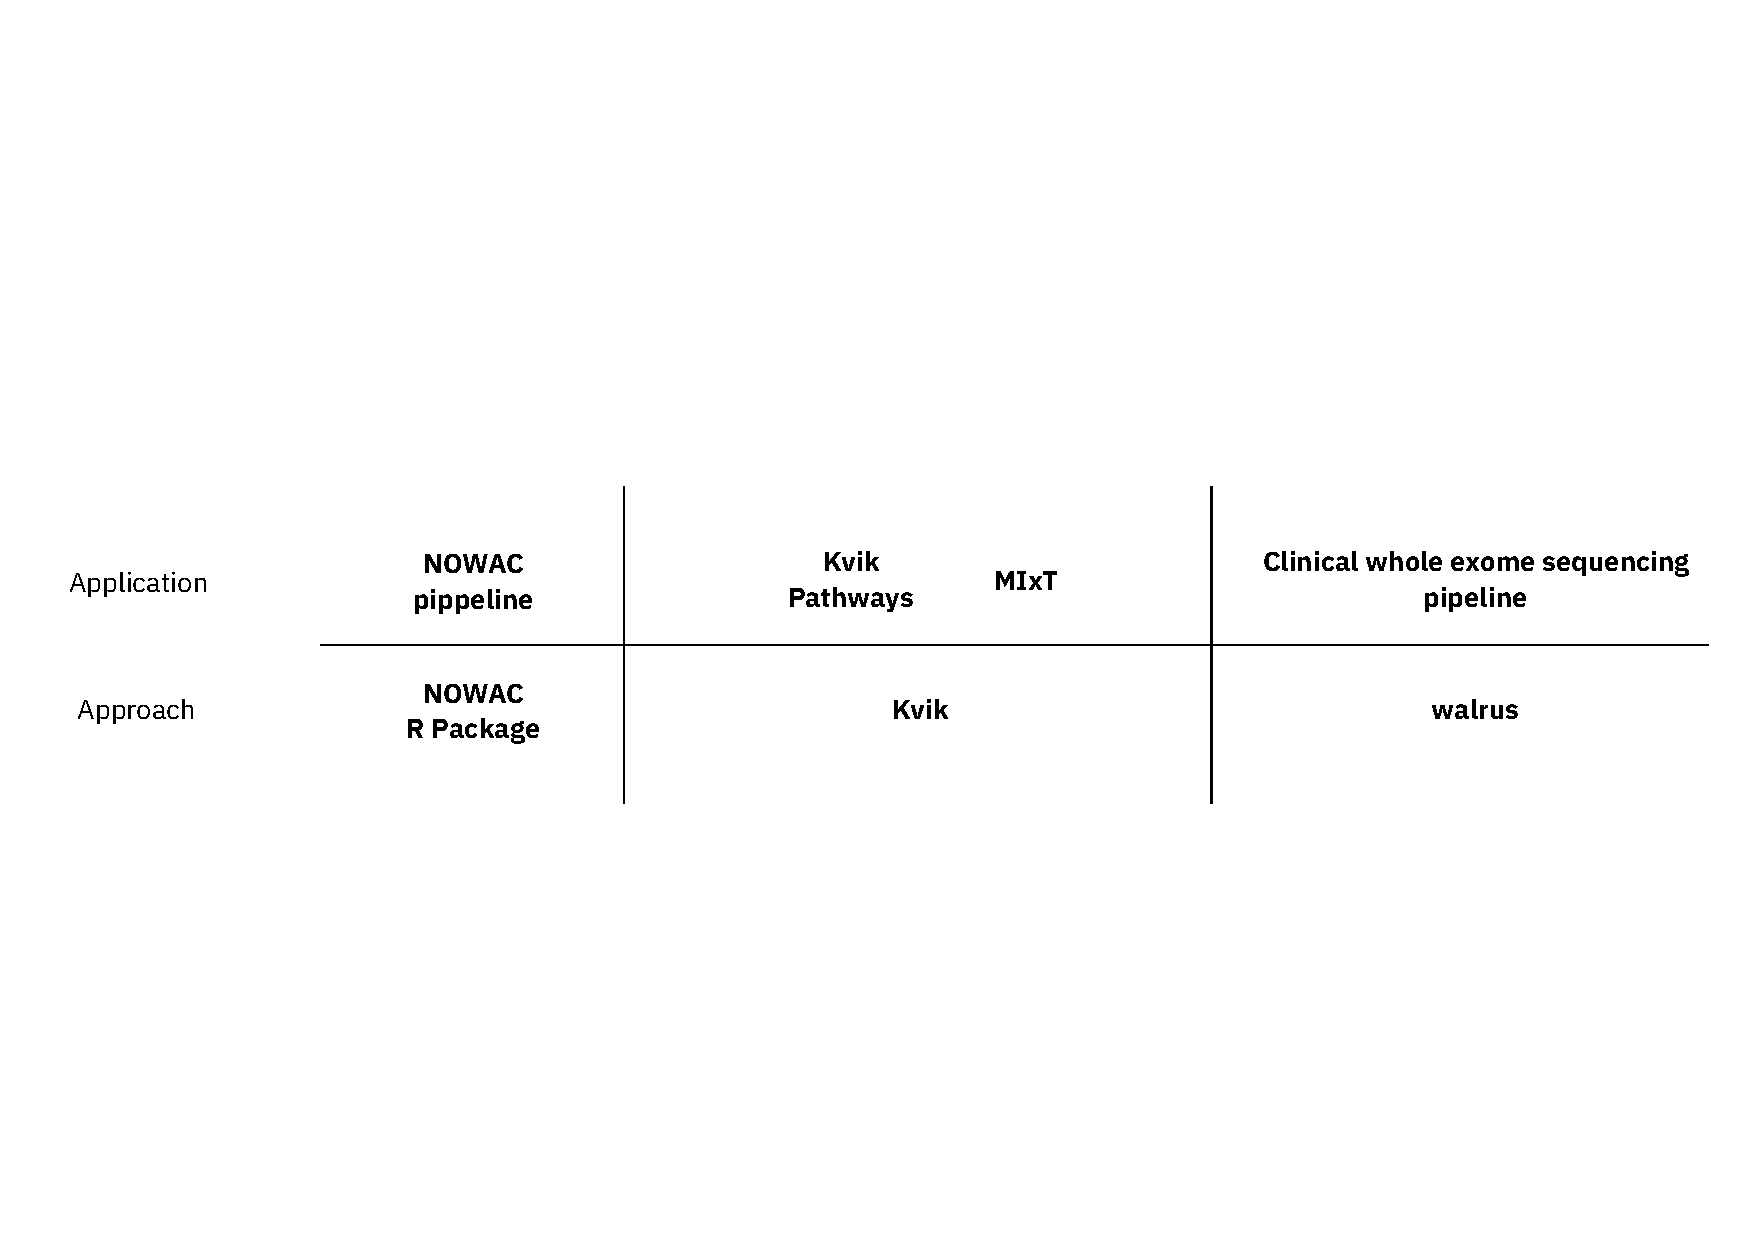
\includegraphics[width=\textwidth]{figures/overall-arch.pdf}
    \caption{The applications and their underlying systems discussed in this
    thesis. } 
    \label{overview-fig}
\end{figure} 

We discuss the different areas separately before highlighting the similarities. 

\textbf{Data Management and Analysis}. 
Modern epidemiological studies now integrate biological datasets with the
traditional questionnaire data and information from public registries.  These
often span multiple biological levels, i.e. different data types and collection
sites. While traditional questionnaire datasets require few specialized
analysis tools because of the relatively simple nature of the data, biological
datasets require specialized tools for reading, analyzing, and interpreting the
data. Package repositories such as Bioconductor provide a wealth of packages for
analyzing these datasets. These packages typically provide analysis tools,
example data, and comprehensive documentation. While the analysis code can be
shared within projects, the datasets are often stored on in-house databases or
shared file systems with specialized permissions, and referenced to in the
analysis scripts. We developed an approach for combining datasets from the
\gls{nowac} cohort with documentation, analysis scripts, and integrates with
registry datasets. This approach makes it a trivial task for new researchers to
start analyzing the different data in our study. 

Inspired by the ecosystem of packages in the R programming
language we developed our approach in the \gls{nowac} package. Users simply
install the package and get access to documentation, datasets, and utility
functions for analyzing datasets related to their area of research. 
In addition we version control both code and the data, making it possible to
track changes over time as the research study evolves. On top of the \gls{nowac}
package we implemented a pre-processing pipelining tool, Pippelinen. Pippelinen
is a web-based interface for running the standardized preprocessing steps before
analyzing gene expression datasets in the \gls{nowac} cohort. 

\textbf{Deep analysis pipelines}. 
Analysis of high-throughput sequencing datasets requires deep analysis pipelines
with a large number of steps that transform raw data into interpretable
results\cite{diao2015building}. There are a large number of tools available to
perform the different processing steps, written in a wide range of programming
languages. The tools, and their dependencies, can be difficult to install, and
they require users to correctly manage a range of input parameters that affects
the output results. With these observations in mind we used software containers
to package the tools we needed for our analyses, one tool per container image.
This made it possible to share the container image between compute systems
without installing any dependencies or additional packages. To keep track of
input parameters as well as the flow of data in a pipeline we designed a
text-based specification for analysis pipelines. This specification includes
information such as input parameters and tool versions. 

This approach was then implemented in walrus, a tool
that lets users create and run analysis pipelines. In addition, it tracks full
provenance of the input, intermediate, and output data, as well as tool
parameters. With \emph{walrus} we have successfully built analysis pipelines to
detect somatic mutations in breast cancer patients, as well as an \gls{rna}-seq
pipeline for comparison with gene expression datasets. 

% LAB: Noe gjentagelser. Blant annet "interface to R" som blir sagt 3 ganger
\textbf{Interactive exploration}. Analysis pipelines and workflows typically
require researchers to browse and explore the final output. In addition it may
be useful to further explore results by modifying analysis parameters to execute
new analyses. As with analysis pipelines there are complete exploration tools as
well as software libraries to develop custom applications. The tools often
require users to import already analyzed datasets but provide interactive
visualizations and point-and-click interfaces to explore the data. Users with
programming knowledge can use the wealth of software packages for visualization
within languages such as R or Python. With a lot modern visualization libraries
created for the web there are also possibilities to develop applications that
target users on any platform. From these observations we wrote an interface to
the R programming language, that would allow us to interface with the wealth of
existing software packages, e.g. the \gls{nowac} package, for biological data
analyses from a point-and-click application. New data exploration applications
could access analyses directly through this interface, removing the previous
decoupling between the two. In addition, to provide reproducible execution
environments we also packaged into software containers that could be easily
deployed and shared. 

This approach was then implemented as a part of \emph{Kvik}, a collection of
packages to develop new data exploration applications. Kvik allows
applications written in any modern programming language to interface with the
wealth of bioinformatics packages in the R programming language, as well as
information available through online databases. We have used Kvik to develop the
\gls{mixt} system for exploring and comparing transcriptional profiles from
blood and tumor samples in breast cancer patients, in addition to applications
for exploring biological pathways. 

\textbf{Parallels}. 
The above approaches to build systems to analyze and explore biological data,
either as interactive applications or batch processing pipelines build on the
same principles.  In all areas we break down the systems in to smaller
composable units, e.g. a tool, and package these into software containers which
are then orchestrated together. These containers are configured and communicate
using open protocols that make it possible to interface with them using any
programming language. We can keep track of the configuration of the containers
and their orchestration using software versioning systems, and provide the
necessary information to reproduce analyses or a complete system. 

\section{Systems Implemented with the X Model/approach/etc.} 
In this section we detail the different systems we have built on top of walrus
and Kvik. 

% LAB: Kommer ikke frem at dette ble gjort som en del av behandling
The first system we built on top of walrus was a pipeline to analyze a patient’s
primary tumor and adjacent normal tissue, including subsequent metastatic
lesions.\cite{walrus} We packaged the necessary tools for the analyses into
software containers and wrote a pipeline description with all the necessary data
processing steps. Some of the steps required us to develop specialized scripts
to generate customized plots, but these were also wrapped in a container. From
the analyses we discovered, among other findings, inherited germline mutations
that are recognized to be among the top 50 mutations associated with an
increased risk of familial breast cancer.

The second analysis pipeline we implemented was to enable comparison of a
\gls{rna}-seq dataset to 
% LAB: microarray
gene expression values collected from the same samples.
The pipeline preprocesses the \gls{rna} dataset for all samples, and generates
transcript quantifications. As with the first pipeline we used existing tools
together with specialized analysis scripts packaged into a container to ensure
that we could reproduce the execution environments. 

%  LAB: Hva med Pippelinen?
The first interactive data exploration application we built was Kvik Pathways.
It allows users to explore gene expression data from the \gls{nowac} cohort in
the context of interactive pathway maps.\cite{pathways} It is a web application
that integrates with the R programming language to provide an interface to the
statistical analyses. We used Kvik Pathways to repeat the analyses in a previous
published project that compared gene expression in blood from healthy women with
high and low plasma ratios of essential fatty acids.\cite{olsen2013plasma}

From the first application it became apparent that we could reuse parts of the
application in the implementation of later systems. In particular, the interface
to run analyses as well as the integration with the online databases could be
implemented as services, packaged into containers, and reused in the next
application we developed. Both of these were designed and implemented in Kvik,
which could then be used and shared later. 

The second application we built the \gls{mixt} web application. A system to
explore and compare transcriptional profiles from blood and tumor samples in
breast cancer patients. The application is built to simplify the exploration of
results from the Matched Interactions Across Tissues (MIxT) study. Its goal was
to identify genes and pathways in the primary breast tumor that are tightly
linked to genes and pathways in the patient blood
cells.\cite{dumeaux2017interactions} The web application interfaces with the
methods implemented as an R package and integrates the results together with
information from biological databases through a simple user interface. 

A third application we developed was a simple re-deployment of the \gls{mixt}
web application with a new dataset. In this application we simply replaced the R
package with a new package that interfaced with different data. All the other
components are reused and highlights the flexibility of the approach. 

% LAB: Her synes jeg du kan si noe om at disse 5 (6) demonstrerer nytten av
% prinsippene i forrige del-kapittel
Combined these systems and applications demonstrate how the X approach is useful
for both batch processing of datasets, as well as interactive applications. 

% Hvordan skal vi knytte inn de under her? Slik som disse systemene er nå er de
% ikke implementert med samme "approach" som jeg har gjort de over. Eller, det
% er jo R-pakker så det er greit, men vi snakker ikke containere. 

% 1. NOWAC package (men merk at data managment challenges/limitations ikke er
% nevnt før). Brukt til å få kontroll over NOWAC data
% 2. Pippelinen. Standardi for NOWAC analyser.
% 6. Bidrag til forskjellige andre paper (den nature methods saken, etc)

\section{Summary of Results} 
% LAB: En figur eller to ville gjort seg her. Men av hva? Screenshot av MIxT?
% Noen performance grafer? Screenshot av Pippelinen? Walrus i bruke for å
% oppdage "zero reads" issue? Eller hva med en figur av alle: dvs nowac package
% -> Pippelinen i walurs -> MIxT i Kvik -> n=1 casen?

We show the viability of our approach through real-world applications in systems
epidemiology and precision medicine. We show that our approach for building
interactive data exploration application, implemented in Kvik, provides the
% LAB: necessary for hva?
necessary interfaces as well as better performance than other related tools. 
% LAB: Her er det andre gang "our approach" er implementert. Også likte jeg
% strukturen for Kvik bedre (our approach for...Kvik...provides...)
We
show that walrus, the implementation of our approach, is suitable for analyzing
precision medicine datasets and we show that the additional steps to track data
provenance does not impose .. overhead. 

We have used walrus to analyze a whole-exome dataset to from a sample in the
McGill Genome Quebec [MGGQ] dataset (GSE58644)\cite{tofigh2014prognostic} to
discover \glspl{snp}, genomic variants and somatic mutations. Using walrus to
analyze a dataset added 10\% to the runtime and doubled the space requirements,
but reduced days of compute time down to seconds when restoring a previous
pipeline configuration. 
% LAB: mulig å si noe om RNA-seq problemene her? Dvs vi brukte approach til å
% finne ut av "zero reads" problemet?

We have used the packages in Kvik to develop a web application, MIxT
blood-tumor, for exploring and comparing transcriptional profiles from blood and
tumor samples in breast cancer patients. 
% LAB: mulig å nevne "den andre" MIxT?
In addition we have used it to build an
application to explore gene expression data in the context of biological
pathways. We show that developing an application using a microservice approach
allows us to reduce database query times down to 90\%, and that we can provide
an interface to statistical analyses that is up to 10 times as fast as
alternative approaches. 

Together the results show that our approach can be used to enable reproducible
data analysis and exploration of high-throughput biological datasets while still
providing the required performance. 
% LAB: jeg savner "easy/ quickly" biten

\section{List of papers} 
This section contains a list of papers along with short descriptions and my
contributions to each paper. 
\capstartfalse
\begin{table}[H]
    \centering
    \begin{tabular}{ | l | p{9.5cm} | }
    \hline
         Title & Kvik: three-tier data exploration tools for flexible analysis
         of genomic data in epidemiological studies \\ \hline
         
         Authors & \textbf{Bjørn Fjukstad}, Karina Standahl Olsen, Mie Jareid,
         Eiliv Lund, and Lars Ailo Bongo \\ \hline
         
         Description & The initial description of Kvik, and how we used it to
         implement Kvik Pathways, a web application for browsing biologicap
         pathway maps integrated with gene expression data from the \gls{nowac}
         cohort. 
         \\ \hline
         
         Contribution & Designed, implemented, and deployed Kvik and Kvik
         Pathways. Evaluated the system and wrote the manuscript. \\ \hline
         
         Publication date & 15 March 2015 \\ \hline 

         Publication venue & F1000 \\ \hline
         
         Citation & \cite{fjukstad2015kvik} \bibentry{fjukstad2015kvik} \\
         \hline 
    \end{tabular}
    \label{p1}

\end{table}
% \hfill 
\begin{table}[H]

    \begin{tabular}{ | l | p{9.5cm} | }
    \hline
         Title & Building Applications For Interactive Data Exploration In
         Systems Biology. \\ \hline
         
         Authors & \textbf{Bjørn Fjukstad}, Vanessa Dumeaux, Karina
         Standahl Olsen, Michael Hallett, Eiliv Lund, and Lars Ailo Bongo.  \\
         \hline
         
         Description & Describes how we further developed the ideas from Paper 1
         into an approach that we used to build the \gls{mixt} web application. 
         \\ \hline
         
         Contribution & 
         Designed, implemented, and deployed Kvik and the \gls{mixt} web
         application.  Evaluated the system and wrote the manuscript. 
         \\ \hline
         
         Publication date & 20 August 2017. \\ \hline  

         Publication venue & The 8th ACM Conference on Bioinformatics,
         Computational Biology, and Health Informatics (ACM BCB) August 20–23,
         2017.  \\
         \hline
         
         Citation & \cite{fjukstad2017building} \bibentry{fjukstad2017building}
         \\ \hline 
    \end{tabular}
    \label{p2}
    
\end{table}
% \hfill 
\begin{table}[H]
    
    \centering
    \begin{tabular}{ | l | p{9.5cm} | }
    \hline
         Title & Interactions Between the Tumor and the Blood Systemic Response
         of Breast Cancer Patients \\ \hline
         
         Authors & Vanessa Dumeaux, \textbf{Bjørn Fjukstad}, Hans E Fjosne,
         Jan-Ole Frantzen, Marit Muri Holmen, Enno Rodegerdts, Ellen
         Schlichting, Anne-Lise Børresen-Dale, Lars Ailo Bongo, Eiliv Lund,
         Michael Hallett.  \\ \hline
         
         Description & Describes the \gls{mixt} system which enables
         identification of genes and pathways in the primary tumor that are
         tightly
         linked to genes and pathways in the patient \gls{sr}. 
         \\ \hline
         
         Contribution & 
         Designed, implemented, and deployed the \gls{mixt} web application.
        Contributed to write the manuscript. 
         \\ \hline
         
         Publication date & 28 September 2017. \\ \hline  

         Publication venue &  PLoS Computational Biology \\ \hline
         
         Citation & \cite{dumeaux2017interactions}
         \bibentry{dumeaux2017interactions}
         \\ \hline 
    \end{tabular}
    \label{p3}
    
    \hfill 

    \begin{tabular}{ | l | p{9.5cm} | }
    \hline
         Title & A Review of Scalable Bioinformatics Pipelines \\ \hline
         
         Authors & \textbf{Bjørn Fjukstad}, Lars Ailo Bongo. \\ \hline
         
         Description & This review survey several scalable bioinformatics
         pipelines and compare their design and their use of underlying
         frameworks and infrastructures.      \\ \hline
         
         Contribution & 
         Wrote the manuscript.  \\ \hline
         
         Publication date & 23 October 2017 \\ \hline  

         Publication venue & Data Science and Engineering 2017. \\ \hline
         
         Citation & \cite{fjukstad2017review} \bibentry{fjukstad2017review} \\
         \hline 
    \end{tabular}
    \label{p4}
\end{table}
\begin{table}[H]
    \centering
    \begin{tabular}{ | l | p{9.5cm} | }
    \hline
         Title & nsroot: Minimalist Process Isolation Tool Implemented With
         Linux Namespaces.  \\ \hline
         
         Authors & Inge Alexander Raknes, \textbf{Bjørn Fjukstad}, Lars Ailo
         Bongo. \\ \hline
         
         Description & Describes a tool for process isolation built using Linux
         namespaces.          \\ \hline
         
         Contribution & Contributed to the
         manuscript, specifically to the literature review and related works.
         \\ \hline
         
         Publication date & 26 November 2017 \\ \hline  

         Publication venue & Norsk Informatikkonferanse 2017. \\ \hline
         
         Citation & \cite{fjukstad2017review} \bibentry{fjukstad2017review} \\
         \hline 
    \end{tabular}
    \label{p5}
\end{table}
\begin{table}[H]
    \centering
    \begin{tabular}{ | l | p{9.5cm} | }
    \hline
         Title & Transcription factor PAX6 as a novel prognostic factor and
         putative tumour suppressor in non-small cell lung cancer \\ \hline
         
         Authors & Yury Kiselev, Sigve Andersen, Charles Johannessen, 
         \textbf{Bjørn Fjukstad}, Karina Standahl Olsen, Helge Stenvold, Samer
         Al-Saad, Tom Dønnem, Elin Richardsen, Roy M Bremnes, and Lill-Tove
         Rasmussen Busund.\\ \hline
         
         Description & This paper explores the possibility of using the PAX6
         transcription factor as a prognostic marker in non-small cell lung
         cancer. 
         \\ \hline
         
         Contribution & Did the analyses to explore association between PAX6
         gene expression and PAX6 target genes. 
         \\ \hline
         
         Publication date & 22 March 2018 \\ \hline  

         Publication venue & Scientific Reports 2018. \\ \hline
         
         Citation & \cite{kiselev2018transcription}
         \bibentry{kiselev2018transcription} \\
         \hline 
    \end{tabular}
    \label{p6}
\end{table}


\begin{table}[H]

    \centering
    \begin{tabular}{ | l | p{9.5cm} | }
    \hline
         Title & Reproducible Data Analysis Pipelines in Precision Medicine \\
         \hline
         
         Authors &  \textbf{Bjørn Fjukstad}, Vanessa Dumeaux, Michael Hallett,
         Lars Ailo Bongo\\ \hline
         
         Description & This paper outlines how we used the container centric
         development model to build walrus. 
         \\ \hline
         
         Contribution & Design, implementation and evaluation of walrus. Wrote
         the manuscript. 
         \\ \hline
         
         Publication date & TBA \\ \hline  

         Publication venue & TBA \\ \hline
         
         Citation & \cite{walrus} \bibentry{walrus} \\
         \hline 
    \end{tabular}
    \label{p6}
\end{table}

% Husk historien: Fra rå data gjennom komplekse analyse pipeliner og helt til
% forskere kan svømme rundt i resultatene. 

\section{Dissertation Plan} 
This thesis is organized as follows. Chapter 2 describes the characteristics of
state-of-the-art biological datasets, the analysis required to extract knowledge
from these, and the available tools and analysis frameworks. Chapter 3 describes
in detail how we use a container centric development model to build a tool,
walrus, to develop and execute deep analysis pipelines. In Chapter 4 we describe
how we used the same model to develop applications to interactively explore
results from statistical analyses.  Finally, Chapter 5 concludes the work and
discusses future directions. 

